\subsection{Zadania}
\setcounter{problem}{0}

\begin{problem}
  Uzasadnij, że jeżeli $\{X_n\}$ są niezależnymi całkowalnymi zmiennymi losowymi o tym samym rozkładzie, a $T$ jest czasem zatrzymania względem filtracji $\set{F}_n=\sigma(X_1,...,X_n)$, takim że $\expected{T}<\infty$, to 
  $$\expected{S_T}=\expected{T}\cdot\expected{X_1}$$
  gdzie $S_n=X_1+X_2+...+X_n$.
\end{problem}

\begin{solution}
  PLAN:
  \begin{center}\scalebox{0.7}{
    \begin{tikzpicture}
      \node (a1) at (0, 0) {martyngał $Y_n=S_n-n\expected{X_1}$};
      \node (a2) at (0, -1.5) {$T$ jest prawie wszędzie skończony};
      \node (a3) at (0, -3) {$Y_{n\land T}$ od pewnego momentu jest stale równy $Y_T$}; 
      \node (a4) at (0, -4.5) {granica $\expected{\lim Y_{n\land T}}=\lim\expected{Y_{n\land T}}$ ma sens};
      \node (a5) at (0, -6) {$\expected{Y_T}=\expected{S_T-T\expected{X_1}}=0$};

      \draw[->] (a1)--(a2);
      \draw[->] (a2)--(a3);
      \draw[->] (a3)--(a4);
      \draw[->] (a4)--(a5);
  \end{tikzpicture}}
  \end{center}

  Jesteśmy w temacie martyngałów, więc możemy chcemy tego użyć.

  Niech $m=\expected{X_1}=\expected{X_n}$ dla każdego $n$. Dobrym początkiem będzie pokazanie, że ciąg $\{S_n-nm\}$ jest martyngałem. W tym celu potrzebujemy całkowalności $[S_n-nm]$, $\set{F}_n$-mierzalności i równości wwo.
  \begin{enumerate}
    \item $[S_n-nm]$ jest całkowalne
    $$\expected{|S_n-nm|}=\expected{\left|\sum X_k-m\right|}\leq\expected{\sum|X_k-m|}=\sum\expected{|X_k-m|}<\infty$$
  \item $[S_n-nm]$ jest $\set{F}_n$-mierzalne, bo jest skończoną sumą $\set{F}_n$-mierzalnych funkcji (wraz z funkcją stałą).
    \item $\expected{S_{n+1}-(n+1)m}{\set{F}_n}=S_n-nm$
      \begin{align*}
        \expected{S_{n+1}-(n+1)m}{\set{F}_n}&=\expected{\sum^{n+1} (X_i-m)}{\set{F}_n}=\\ 
                                            &=\expected{X_{n+1}-m}{\set{F}_n}+\sum(X_i-m)=\\ 
                                            &=\expected{X_{n+1}}-m+S_n-nm=m-m+S_n-nm=S_n-nm
      \end{align*}
  \end{enumerate}

  Dla uładnienia zapisu niech $Y_k=n=S_n-n\cdot m$, wtedy $\{Y_n\}$ jest martyngałem względem filtracji jak w zadaniu. 
  Z twierdzenia Dooba o zatrzymaniu wiemy, że
  $$\expected{Y_{n\land T}}=\expected{Y_1}=S_1-m=0$$
  Będziemy chcieli przejść z $n$ do granicy, do czego potrzebujemy aby $\prob{T\geq n}\to 0$, bo wówczas ciąg $X_{n\land T}$ zbiega prawie wszędzie do $X_T$. Wystarczy przypomnieć sobie ostatnie zadanie z poprzedniej listy, aby dostać
  $$\expected{T}=\sum_{k\geq 0}\prob{T>k}<\infty$$
  czyli w pewnym momencie wyrazu muszą być dowolnie blisko $0$, czyli faktycznie $\prob{T\geq n}\to 0$.

  Przechodząc z $n$ do granicy dostajemy
  $$\expected{Y_T}=\expected{\lim Y_{n\land T}}=\lim\expected{Y_T}=0$$
  ponieważ $Y_{n\land T}$ zbiega do $Y_T$, więc od pewnego momentu jest stały i granica ma sens.

  Rozbijając więc $Y_T$ na wzór podany wyżej, dostajemy
  $$0=\expected{Y_T}=\expected{S_T-Tm}=\expected{S_T}-\expected{T\expected{X_1}}$$
  czyli
  $$\expected{S_T}=\expected{T\expected{X_1}}=\expected{X_1}\expected{T}$$
  tak jak chcieliśmy.

  {\large\color{red}Można też zapisać najpierw $\expected{|S_T|}=\sum_{t=1}^\infty\expected{|S_T|\mathds{1}_{\{T=t\}}}$. JEDNAK BŁĄD Z $\prob{T\geq k}\to 0$ bo to niekoniecznie musi być prawdą - trzeba by używać $\expected{S_{n\land T}}$} 
\end{solution}

\begin{problem}
  Rzucamy kostką tak długo, aż pięciokrotnie wyrzucimy szóstkę. Znajdź średnią wartość sumy wyrzuconych oczek.
\end{problem}

\begin{solution}
  Zadania wygląda bardzo podobnie jak równość udowadniana wyżej. Chcemy tylko znaleźć martyngał i czas zatrzymania.

  Niech $X_i$ będzie liczbą oczek wyrzuconych w $i$-tym rzucie, a $S_n=\sum_{k=1}^nX_i$ będzie sumą oczek wyrzuconych w pierwszych $n$ rzutach. Oczywiście, $X_i$ mają ten sam rozkład jednostajny na zbiorze $\{1,...,6\}$ i są od siebie niezależne. Zdefiniujmy teraz funkcję
  $$T=\inf \{n\;:\;(X_1,...,X_n)\;\text{posiada 5 szóstek}\}$$
  która jest czasem zatrzymania względem filtracji $\mathds{F}=\{\set{F}_n\}$, $\set{F}_n=\sigma(X_1,...,X_n)$, bo jej definicja opiera się wyłącznie na informacjach o $X_1,...,X_n$.

  Korzystając więc z poprzedniego zadania, dostajemy
  $$\expected{S_T}=\expected{T}\expected{X_1}=\expected{T}\cdot\frac{7}{2}$$
  i jedynym problemem jest obliczenie 
  $$\expected{T}=\sum_{n\geq0}n\prob{T=n}.$$
  Oczywiście, dla $\prob{T=1}=\prob{T=4}=0$, a w pozostałych przypadkach jest to stosunek wszystkich ciągów długości $n-1$ które posiadają dokładnie $4$ szóstki do ilości wszystkich ciągów posiadających co najwyżej $4$ szóstki.
\end{solution}

\begin{problem}
  Niech $\{X_n\}$ będzie niesymetrycznym spacerem losowym na $\Z$ (tzn. $X_n=\sum_{k=1}^n\xi_k$, gdzie $\xi_k$ są iid takie, że $\prob{\xi_k=1}=1-\prob{\xi_k=-1}=p\neq\frac{1}{2}$) i niech $T=\min\{n\;:\;X_n=-j\text{ lub }X_n=k\}$ dla ustalonych $k,j>0$.
  \begin{enumerate}[label=(\alph*)]
    \item Pokaż, że $M_n=X_n+n(1-2p)$ jest martyngałem.
    \item Wykorzystując twierdzenie Dooba oblicz $\expected{T}$.
  \end{enumerate}
\end{problem}

\begin{solution}$ $
  Filtrem u mnie będzie $\set{F}_n=\sigma(\xi_1,...\xi_n)$.

  \begin{enumerate}[label=(\alph*)]
    \item Wypadałoby pokazać, że $M_n$ jest całkowalne, czyli
      \begin{align*}
        \expected{|M_n|}&=\expected{|X_n+n(1-2p)|}\leq \expected{|X_n|}+n(1-2p)=\\ 
                        &=\expected{|\sum\xi_k|}+n(1-2p)\leq \sum\expected{|\xi_k|}+n(1-2p)<\infty 
      \end{align*}
      Jest $\set{F}_n$-mierzalne bo jest kombinacją funkcji $\set{F}_n$-mierzalnej z funkcją stałą. Pozostaje warunek z wwo:
      \begin{align*}
        \expected{M_{n+1}}{\set{F}_n}&=\expected{X_{n+1}+(n+1)(1-2p)}{\set{F}_n}=\\ 
                                     &=\expected{X_{n+1}}{\set{F}_n}+(n+1)(1-2p)=\\ 
                                     &=\expected{\sum^{n+1}\xi_k}{\set{F}_n}+(n+1)(1-2p)=\\ 
                                     &=\sum^{n+1}\expected{\xi_k}{\set{F}_n}+(n+1)(1-2p)=\\ 
                                     &=X_n+n(1-2p)+\expected{\xi_{n+1}}{\set{F}_n}+(1-2p)=\\ 
                                     &=X_n+n(1-2p)=M_n
      \end{align*}
    \item To jest tak samo jak w zadaniu $1$, tylko trzeba pokazać, że z prawdopodobieństwem $1$ w kończenie wielu krokach dojdziemy do $-j$ lub $k$. A tutaj można użyć Borel-Cantalliego :3
  \end{enumerate}
\end{solution}

\begin{problem}
  Niech $\{M_n\}$ będzie nieujemnym martyngałem. Pokaż, że dla $m>n$, $\{M_n=0\}\subseteq\{M_m=0\}$ prawie wszędzie.
\end{problem}

\begin{solution}
  Rozważmy zbiór $A=\{M_n=0\}\in\set{F}_n$. Ponieważ $\{M_n\}$ jest martyngałem, to na poprzedniej liście pokazywaliśmy, że
  $$\expected{M_m}{\set{F}_n}=M_n.$$
  W takim razie mamy
  \begin{align*}
    0=\expected{M_n\mathds{1}_A}=\expected{\expected{M_m}{\set{F}_n}\mathds{1}_A}=\expected{M_m\mathds{1}_A}
  \end{align*}
  Ponieważ $M_m\geq0$ oraz $\int_AM_md\prob=0$, to $M_m=0$ prawie wszędzie na zbiorze $A$. Czyli 
  $$A\subseteq\{M_m=0\}$$ 
  prawie wszędzie.

  %  Rozważmy zmienną losową
%  $$T=\inf\{n\;:\;(\forall\;k\geq n)\;M_k=0\}$$
%
%
%  Rozważmy zbiór
%  $$A=\{\omega\;:\;M_n(\omega)\neq 0\;i\;M_m(\omega)=0\}$$
%  chcemy pokazać, że $\prob{A}=0$.
%
%  Zauważmy, że $A$ zawiera informacje o $\omega$ pojawiające się tylko w $\sigma(M_1,...,M_m)$.
%  \begin{align*}
%    \prob{A}&=\expected{\mathds{1}_A}
%  \end{align*}
\end{solution}

\begin{problem}
  Niech $\mathds{F}=\{\set{F}_n\}$ będzie filtracją.
  \begin{enumerate}[label=(\alph*)]
    \item Pokaż, że dla każdych $m,n\in\N$, $m<n$ i zdarzenia $A\in\set{F}_m$ zmienna losowa
      $$\tau=m+(n-m)\mathds{1}_A$$
      jest $\mathds{F}$-czasem zatrzymania.
    \item Niech $\{X_n\}$ będzie $\mathds{F}$-adaptowalnym ciągiem całkowalnych zmiennych losowych takim, że
      $$\expected{X_\tau}=\expected{X_0}$$
      dla każdego skończonego czasu zatrzymania $\tau$. Pokaż, że $\{X_n\}$ jest $\mathds{F}$-martyngałem.
  \end{enumerate}
\end{problem}

\begin{solution}$ $

  \begin{enumerate}[label=(\alph*)]
    \item Musimy sprawdzić, że zdarzenie $\{\tau=k\}\in\set{F}_k$. Od razu widzimy, że $\tau$ ma jedynie dwie możliwe wartości:
      $$\tau(\omega)=\begin{cases}m & \omega\not\in A\\n & \omega\in A\end{cases}$$
      Zacznijmy od $\{\tau =m\}$. Ale tak jak wyżej napisaliśmy, to zachodzi tylko dla $\omega\not\in A$, czyli $\{\tau=m\}=A^c\in\set{F}_m$, bo $A\in\set{F}_m$.

      Z kolei $\{\tau=n\}=A$, a wiemy, że $A\in\set{F}_m\subseteq\set{F}_n$ bo $m<n$.

      W takim razie $\tau$ zachowuje się jak bardzo dziwny czas zatrzymania.
    \item PLAN na ten podpunkt jest taki (pokazujemy $\expected{X_{m+1}}{\set{F}_m}=X_m$):
      \begin{center}\scalebox{0.6}{
        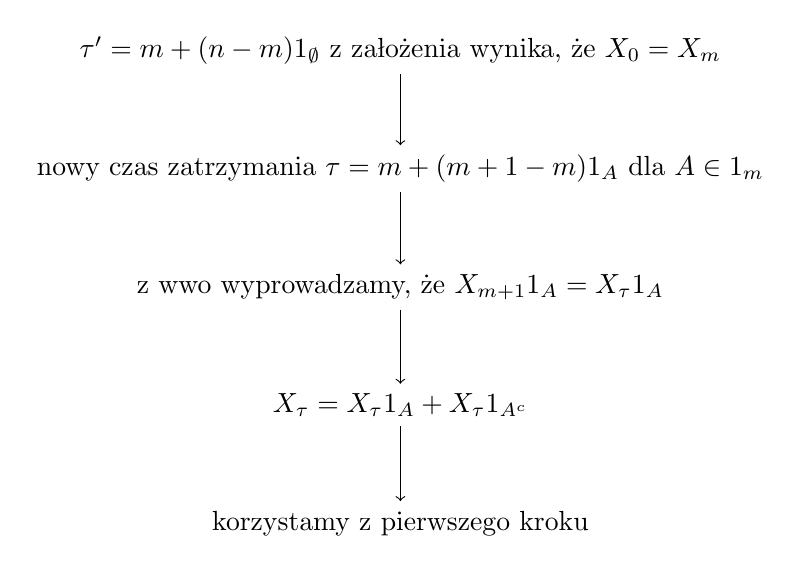
\begin{tikzpicture}
          \node (a1) at (0, 0) {$\tau'=m+(n-m)\mathds{1}_\emptyset$ z założenia wynika, że $\expected{X_0}=\expected{X_m}$};
          \node (a2) at (0, -1.5) {nowy czas zatrzymania $\tau=m+(m+1-m)\mathds{1}_A$ dla $A\in\mathds{1}_m$};
        \node (a3) at (0, -3) {z wwo wyprowadzamy, że $\expected{X_{m+1}\mathds{1}_A}=\expected{X_\tau\mathds{1}_A}$ };
        \node (a4) at (0, -4.5) {$\expected{X_\tau}=\expected{X_\tau\mathds{1}_A}+\expected{X_\tau\mathds{1}_{A^c}}$};
        \node (a5) at (0, -6) {korzystamy z pierwszego kroku};
          \draw[->] (a1)--(a2);
          \draw[->] (a2)--(a3);
          \draw[->] (a3)--(a4);
          \draw[->] (a4)--(a5);
      \end{tikzpicture}}
      \end{center}

      Zaczniemy od wprowadzenia czasu zatrzymania
      $$\tau'=m+(n-m)\mathds{1}_\emptyset$$
      dla dowolnego $n>m$ i użycia założenia z tego punktu, by otrzymać
      $$\expected{X_0}=\expected{X_{\tau'}}=\expected{X_{\tau'}\mathds{1}_\emptyset}+\expected{X_{\tau'}\mathds{1}_{\emptyset^c}}=\expected{X_m\mathds{1}_\Omega}=\expected{X_m}$$
      gdyż $\expected{X_{\tau'}\mathds{1}_\Omega}=\int_\Omega X_{\tau'(\omega)}(\omega)=\int X_m$ - całkujemy tę część tylko po zbiorze gdzie $\tau'=m$.

      Rozważamy teraz czas zatrzymania
      $$\tau=m+(m+1-m)\mathds{1}_A=m+(m+1)\mathds{1}_A$$
      dla dowolnego $A\in\set{F}_m$.

      Z jednej strony wiemy, że
      $$\expected{\expected{X_{m+1}}{\set{F}_m}\mathds{1}_A}=\expected{X_{m+1}\mathds{1}_A}=\expected{X_\tau\mathds{1}_A}$$
      A z drugiej
      $$\expected{X_0}=\expected{X_\tau}=\expected{X_\tau\mathds{1}_A}+\expected{X_\tau\mathds{1}_{A^c}}=\expected{X_{m+1}\mathds{1}_A}+\expected{X_m\mathds{1}_{A^c}}$$
      czyli korzystając z $\expected{X_0}=\expected{X_m}$ mamy
      $$\expected{X_{m+1}\mathds{1}_A}=\expected{X_0}-\expected{X_m\mathds{1}_{A^c}}=\expected{X_m}-\expected{X_m\mathds{1}_{A^c}}=\expected{X_m(1-\mathds{1}_{A^c}}=\expected{X_m\mathds{1}_A}$$
      i to już wystarczy, bo $X_m$ jest mierzalne względem $\set{F}_m$ ponieważ jest $\mathds{F}$-adaptowalne.
  \end{enumerate}
\end{solution}

\begin{problem}
  Niech $\{M_n\}$ będzie nieujemnym martyngałem o wartościach całkowitym takim, że $M_0=m\geq1$, $M_n-M_{n-1}\leq 1$ oraz $M_n\to 0$ p.w.. Pokaż, że dla $k\geq m$,
  $$\prob{\sup_{n\in\N}M_n\geq k}=\frac{m}{k}$$
\end{problem}

\begin{solution}
  Zacznijmy od rozważenia co znaczy, że $\sup_{n\in\N}M_n\geq k$. Moim skromnym zdaniem jest to powiedzenie, że $M_n$ dojdzie do $k$. Wiemy, że w każdym przejściu z $M_n$ do $M_{n+1}$ możemy skoczyć w górę o nie więcej niż $1$, a w dół możemy skakać aż do $0$.

  PLAN na to zadanie jest taki:
  \begin{center}\scalebox{0.6}{
    \begin{tikzpicture}
      \node (a1) at (0, 0) {czas zatrzymania $T=\inf\{n\;:\;M_n\geq k\}$};
      \node (a2) at (0, -1.5) {$\sup{M_n}\geq k\iff T<\infty$, więc $\prob{\sup M_n\geq k}=\prob{T<\infty}$};
      \node (a3) at (0, -3) {twierdzenie Dooba daje $m=\expected{M_0}=\expected{M_{n\land T}}$};
      \node (a4) at (0, -4.5) {$\lim_n M_{n\land T}$ będzie $M_T=k$ jeśli $T<\infty$ i $M_n$ wpp.};
      \node (a5) at (0, -6) {$M_{n\land T}\in\{0,...,k\}$};
      \node (a6) at (0, -7.5) {$\prob{M_{n\land T}<k}\to 0$, bo jeśli $T=\infty$ to $M_n\to 0$, a jeśli $T<\infty$, to $M_{n\land T}\to M_T=k$ jest stałe od pewnego momentu};
      \node (a7) at (0, -9) {$\lim \prob{M_{n\land T}=k}=\prob{T<\infty}$};
      \node (a8) at (0, -10.5) {$m=\sum_{0\leq i\leq k} i\prob{M_{n\land T}}\to k\prob{T<\infty}$};

      \draw[->] (a1)--(a2);
      \draw[->] (a2)--(a3);
      \draw[->] (a3)--(a4);
      \draw[->] (a4)--(a5);
      \draw[->] (a5)--(a6);
      \draw[->] (a6)--(a7);
      \draw[->] (a7)--(a8);
  \end{tikzpicture}}
  \end{center}

  Spróbujmy zobaczyć co się stanie, jeśli wplączemy w to zadanie czas zatrzymania
  $$T=\inf\{n\;:\;M_n\geq k\}$$
  to możemy zauważyć, że 
  $$\prob{\sup_{n\in\N}M_n\geq k}=\prob{T<\infty}=\prob{M_{n\land T}=k}$$
  ponieważ $T<\infty$ oznacza, że zbiór $\{n\;:\;M_n\geq k\}$ jest niepusty.

  Z twierdzenia Dooba wiemy, że
  $$m=\expected{M_0}=\expected{M_{n\land T}}$$
  zauważmy, że jeżeli $T(\omega)<\infty$, to $M_{n\land T}(\omega)=M_{T(\omega)}(\omega)=k$, a jeśli $T(\omega)=\infty$, to $M_{n\land T}(\omega)=M_n(\omega)$. 

  Oznacza to, że jeśli $M_{n\land T}\geq k$, to $M_{n\land T}=k$ i jest od tego momentu funkcją stałą. W takim razie
  $$m=\expected{M_{n\land T}}=\sum_{j=0}^kj\prob{M_{n\land T}=j}=k\cdot\prob{M_{n\land T}=k}+\sum_{j=0}^{k-1}j\prob{M_{n\land T}=j}$$
  przechodząc teraz z $n$ do granicy, albo $M_{n\land T}=k$ albo $M_{n\land T}=M_n$ i w obu przypadkach $\prob{M_{n\land T}=j}=0$ dla $j<k$ (bo $M_n\to 0$). W takim razie, po przejściu do granicy z $n$ zostaje nam
  $$m=k\cdot\prob{\sup_{n\in\N}M_n\geq k}$$
  i to jest to co chcieliśmy.
\end{solution}

\begin{problem}
  Niech $Y_k$ będą iid takie, że $\prob{Y_k\in\{-1,0,1\}}=1$ oraz $\expected{Y_k}=0$. Niech $S_0=0$, $S_n=Y_1+...+Y_n$. Dla $k\in\N$ rozważmy moment zatrzymania
  $$T_{-k}=\inf\{n\;:\;S_n=-k\}.$$
  Znajdź rozkład zmiennej losowej
  $$\sup_{n\leq T_{-k}}S_n$$
\end{problem}

\begin{solution}
  Zmienna losowa
  $$\sup_{n\leq T_{-k}}S_n$$
  pyta, jak wysoko możemy dojść, jeśli zatrzymamy się przy pierwszym dojściu do $-k$.

  Popatrzmy teraz na $\prob{Y_k=1}$. Oznaczając $\prob{Y_k=0}=p$ mamy
  $$0=\expected{Y_k}=\prob{Y_k=1}-\prob{Y_k=-1}$$
  $$\prob{Y_k=1}=\prob{Y_k=-1}=\frac{1-p}{2}$$
\end{solution}
